\chapter{Background} \label{c:backgrnd}

\section{Probabilistic Graphical Models} \label{c:pgms}

Probabilistic graphical models (PGMs) or structured probabilistic models can be used to describe, formalize and model neural learning architectures \cite{Goodfellow-et-al-2016-Book} \cite{Petrovici2016}.

They can capture the basic probabilistic structure of data, which makes a lot of data-related task feasible, such as \cite{Goodfellow-et-al-2016-Book}:
\begin{itemize}

\item Density estimation: Assigning a data sample $x$ an estimate of its true probability density $p(x)$ (e.g. indicating unusual data).

\item Denoising: Given a perturbed or noisy input $\widetilde{x}$,  estimating the original data sample $x$

\item Missing value imputation: Given a partial input sample of $x$, it returns the most probable completion of the mission values to return $x$ ( e.g. inferring a label of data sample).

\item Sampling: Generating data samples $x$ drawn from the data distribution $p(x)$. 

\end{itemize}  

PGMs facilitate the process of modeling the probability distribution by using graphs to describe the probability distribution over the interactions of its random variables (RVs).
A node in the graph represents a RV and an edge a direct interaction between two RVs.
This allows a less complex description of the probability density with basic factors over interacting RVs instead of modelling the probability density over all RVs. 

How to build a PGM and set the parameters for a given problem is still an topic of active research \cite{Ghahramani2002}\cite{Zhou2007}.
There exist different approaches such as the SGS algorithm \cite{Zhou2007} or EM algorithms\cite{Ghahramani2002}, but in the following we will use Boltzmann machines and the contrastive divergence algorithm, to build up and set the parameters in a PGM (see Chapter \ref{c:bms}).

PGMs can be be divided into two basic categories, models with directed graphs and model with undirected graphs.


\subsection{Bayesian network} \label{c:bayesnet}

Bayesian networks or belief networks are directed acyclic graphs, in which random variables are represented by nodes and their causal dependencies are represented by (directed) edges/connections \cite{Faltin2007} \cite{Goodfellow-et-al-2016-Book}. 
It poses a way to depict a probability distribution factorized by repeatedly applying the Bayes rule.

A connection from $x_i$ to $x_j$ represents a conditional probability distribution from $x_j$ dependend on $x_i$, and $x_i$ is called the parent of its child $x_j$:

\[
p(x_j | x_i) .
\]


If there exists a path from node $x_n$ to $x_k$ then $x_n$ is called an ancestor of $x_k$, and $x_k$ an descendant of $x_n$. 

As well as the graph structure, which is often called the "qualitative" part of the models, the "quantitative" part has to be determined as well.
The quantitative parameters are described by the local conditional probability distribution at each node given its parents.
A sample network with the qualitative part as well as the quantitative part can be seen in Figure \ref{fig:bayesnet}. 

\begin{figure}[h]
	\centering
	\begin{subfigure}[t]{.33\textwidth}
  		\centering
  		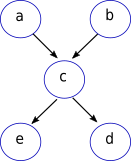
\includegraphics[width=.6\linewidth]{imgs/bayesnet1.png}
  		\caption{A Bayesian with 5 RVs.}
  		\label{fig:sub1}
	\end{subfigure}%
	\begin{subfigure}[t]{.33\textwidth}
  		\centering
  		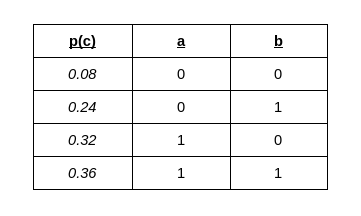
\includegraphics[width=.9\linewidth]{imgs/bayesnet2.png}
  		\caption{Tabular conditional probability $p(c |a , b)$.}
  		\label{fig:sub2}
	\end{subfigure}
	\begin{subfigure}[t]{.33\textwidth}
  		\centering
  		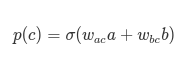
\includegraphics[width=.7\linewidth]{imgs/bayesnet3.png}
  		\caption{Conditional probability $p(c |a , b)$ given by a function over $a,b$.}
  		\label{fig:bayesnet}
	\end{subfigure}
	\caption{A sample Bayesian network with 5 binary nodes. (a) In the network RV $c$ is directly dependent on $a$, $b$ and thus $c$ is the child of its parents $a$, $b$. The RVs $d$, $e$ are the children of $c$. Since there is a path from $a$ to $e$, $a$ is an ancestor of its descended $e$. (b) The conditional probability of $p(c |a , b)$ in a tabular form. Another variant of the conditional probability $p(c |a , b)$ is given in (c). The probability is defined by the parameters $w_{ac}$, $w_{bc}$, and due to the sigmoid activation function $\sigma$ a network with such probability functions is called sigmoid belief network.}
	\label{fig:test}
\end{figure}

This is consistent with with the Markov property, since each node is only depend on its direct parents:

\[
p(x_i | x_{\setminus i}) = p(x_i | parents(x_i) ),
\]

where $x_{\setminus i} = \textbf{z} \setminus x_i$ and $\textbf{z} = (x_1, ... , x_n)$ is the state of the model.


A Bayesian network contains a simple conditional independence assertion, i.e. each variable is, given its parents, independent on all non descendants:

\[
p(\textbf{z}) = \prod_{x_i \in \textbf{z}} p(x_i | x_{\setminus i}) = \prod_{x_i \in \textbf{x}} p(x_i | parents(x_i) ) .
\]

This reduction provides (i.a from a computational perspective) an efficient way for learning/ parameter estimation and inference.
Given some observed variables, the evidences, the network can be used to compute the posterior probabilities and infer the most likely state of the hidden/ unobserved variables.
This process of computing the posterior distributions given the evidences is called probabilistic interference.

Thus a Bayesian network can be seen as a tool to simplify and apply the Bayes rule to complex problems.   

\subsection{Markov Random Field} \label{c:markovnet}

In contrast to Bayesian networks, Markov random fields are undirected graphical models, in which random variables are also represented by nodes but edges in this case indicate conditional dependencies \cite{Goodfellow-et-al-2016-Book}\cite{murphy2012machine}.
If two nodes $x_i$ and $x_j$ are connected by a edge, they are called each others neighbours.
Given all of their neighbours, two nodes $x_k$ and $x_m$ are independent on each other.
Thus an MRF can be seen as a model of the joint probabilities of RVs (see Fig. \ref{fig:markovnet1}).

As a result to reduce the complexities and redundancies of the probability distribution, instead of defining one probability distribution over all RVs, this allows a factorization of the probability distribution into fully connected partial graphs, so-called cliques:

\[
p(\textbf{z}) = \frac{1}{Z} \prod \phi (z_k)  ,
\]

where $Z$ is the normalization factor, so that $p(\textbf{z})$ is a valid probability distribution with $\sum_{\textbf{z}} p(\textbf{z}) = 1$ ($ \Rightarrow Z = \sum_z \prod \phi (z_k) $) and $\phi (z_k)$ is the partition function of the clique/ partial graph $z_k$.

The partition function $\phi (z_k)$ defines the potential of a clique, which indicates the likelihood of a state in the clique to be present.
The higher the clique potential of a state the more likely is that clique-state.
The clique potential for each state always has to be greater or equal to zero, but a common, computational beneficial choice is to represent each state with is purely positive value.

\begin{figure}
	\centering
	\begin{subfigure}[t]{.5\textwidth}
  		\centering
  		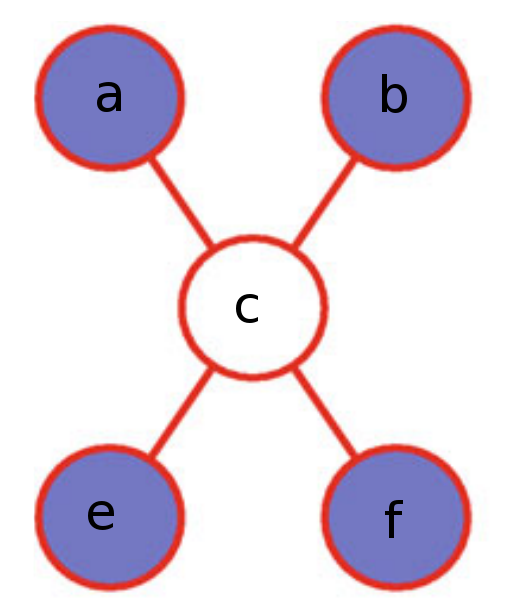
\includegraphics[width=.5\linewidth]{imgs/markovnet1.png}
  		\caption{A Markov network with with 5 nodes.}
  		\label{fig:markovnet1}
	\end{subfigure}%
	\begin{subfigure}[t]{.5\textwidth}
  		\centering
  		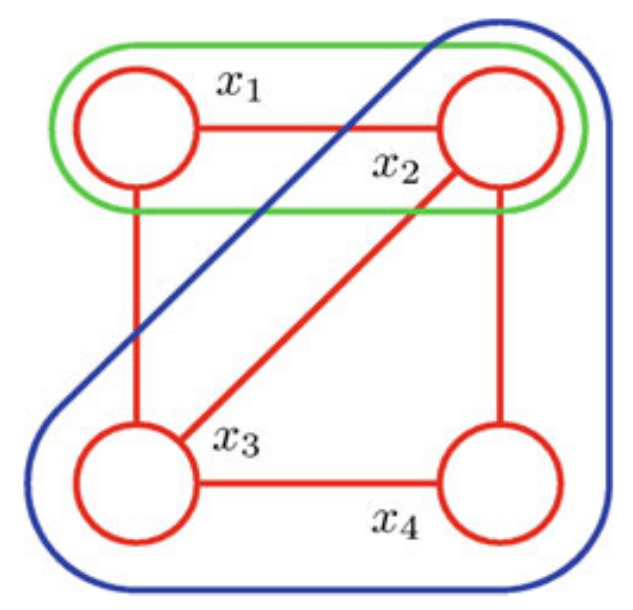
\includegraphics[width=.5\linewidth]{imgs/markovnet2.png}
  		\caption{Cliques in a Markov network}
  		\label{fig:markovnet2}
	\end{subfigure}
	\caption{(a) A Markov network with 5 nodes. The white node is dependent on all connected nodes (blue nodes). Given the blue nodes the white node is independent on any other node in the network. Given the white node all the blue nodes are independent on each other. (b) Two cliques in a Markov network. The blue clique is maximal, since no vertex can be added, which is fully connected to all others in the blue clique. The green one is not maximal, since the node $x_3$ could be added \cite{bishop2013pattern}.}
	\label{fig:markovnet}
\end{figure}


Usually the maximal (sized) cliques are chosen, since they contain all smaller sub-cliques and allow a finer factorization over those sub-cliques.
But depending on the concrete modelled problem, smaller clique sizes may be useful as well, e.g. Boltzmann machines usually are modelled with cliques of size two (see Fig. \ref{fig:markovnet2}).




\subsection{Energy-Based Models} \label{c:ebms}

One convenient way to model the clique potentials is to use an energy function $E(z_k)$ \cite{Goodfellow-et-al-2016-Book}: 

\[
\phi(z_k) = exp(- E(z_k))
\]

Models with exponentials over energy functions are called energy-base models (EBMs).

This is useful since, due to $exp(z_n)exp(z_m) = exp(z_n+z_m)$, the Energy of the complete graph can be decomposed into the sum of the energy of all cliques.
Because the exponential function is always positive ($exp(z) > 0$), the probability for each state is guaranteed to be greater than zero. 
This offers the freedom of choice of an arbitrary energy function $E(z_k)$, which can simplify optimization. 

A probability distribution given by an EBM is also called Boltzmann distribution, due to the similarity to statistical mechanics of gases in thermal equilibrium (and this is also where the Boltzmann machine get its name as presented in Chapter \ref{c:bms} ).

\subsection{Sampling} \label{c:sampling}

Often calculating the exact probability distribution or marginal distributions is a computational inefficient or untraceable problem \cite{Goodfellow-et-al-2016-Book} \cite{Petrovici2016}.
Sampling is a probabilistic solution to this problem, as it allows to approximate the target distribution nearly arbitrarily exact, and also turns calculating marginal probabilities into a by-product.  
An exemplary sampling of a Gaussian distribution is given in Figure \ref{fig:Sampling}.

Sampling can be described as the selection of a subset of individuals from a distribution to estimate properties of the complete distribution.
To select a representative subset, the samples have to be unbiased of external influences, such as the the sampling procedure or problems in data collection.
This can be particularly hard since it may need infinite data, computational or temporal resources.
This where graphical models are especially useful, since they often facilitate the task of drawing samples from a distribution.

\begin{figure}
	\centering
    	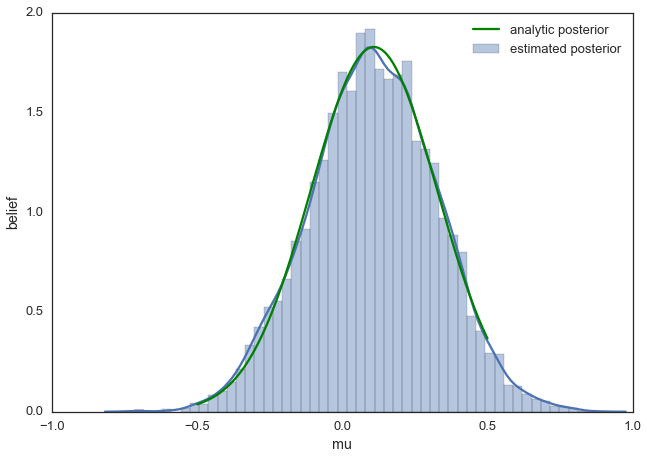
\includegraphics[width=0.4\textwidth]{imgs/sampling.png} 
    \caption{Sampling a Gaussian distribution. The number of samples in an interval approximates the true density function. As more samples are drawn, the approximation of the density function will be more exact \cite{sampleFD}.}
	\label{fig:Sampling}
\end{figure}



\paragraph{Ancestral Sampling} For directed graphical models, such a Bayesian networks, there is a simple and efficient procedure called ancestral sampling, which can produce samples from the probability distribution represented by the model \cite{Goodfellow-et-al-2016-Book}. 
The basic idea is to sort the variables $x_n$ in the graph into a topological ordering, so that for all $i$ and $j$, $j$ is greater than $i$ if $x_i$ is a descendant of $x_j$. The variables can then be sampled in this order.

The topological sorting operation guarantees that the conditional distributions are valid and one can sample from them in order.

\paragraph{Markov Chain Monte Carlo} If the probability distribution is represented by an undirected model, Markov Chain Monte Carlo (MCMC) methods can be used \cite{Goodfellow-et-al-2016-Book}. 
MCMC methods interpret the model as a Markov chain, and work best in an irreducible and aperiodic chain, that is when no state in the undirected model has zero probability.

The basic idea is to begin in a state $z$ with some arbitrary value. 
Then for some time $z$ is repeatedly randomly updated using the, by the model given, transition distribution $T(z',z)$. 
Given enough update steps (possibly an infinite number) the network states will have reached a distribution, which does not change any more (even so the individual states might do, the relative number of time spend in on state becomes constant).
Such a distribution is referred to as stationary distribution or equilibrium distribution (due to its similarity to particle physics).
Eventually $z$ becomes a fair sample of $p(z)$, which is equivalent to the stationary distribution of the Markov chain.

To get more than one sample, one can run more Markov chains in parallel, each initialized with a random starting state. 
Another method is to run only one Markov chain, run it for some time to allow the Markov chain to reach its equilibrium, and than take samples after different timesteps.
Those approaches need the Markov chain to reach its equilibrium distribution, which is usually done, by letting it run for some burn in time.
But there is no guaranty, that the Markov chain has settled in the given timespan.    
Another problem with the second approach is, that since it can be hard to escape probable states, and when not run for an infinite timespan, more likely states can be over represented and less likely states under represented, if they did not occur or over represented if they did occur.  

\paragraph{Gibbs sampling} Gibbs sampling is a commonly used MCMC algorithm \cite{Goodfellow-et-al-2016-Book}. The basic idea to perform the transition from one state to another in accordance with $T(z',z)$ is, to sample a single variable $x_i$ only conditioned on its neighbours. 
Several variables can be sampled at the same time as long as they are conditionally independent given all of their neighbours.

\section{Neural Networks} \label{c:NNs}

In this section we will examine the foundations of natural and artificial neural networks (NNs).
At first we will look at the mechanism behind natural neural networks in the brain.
We will then describe different artificial models, starting with models working at discrete time steps and then models, which work in continuous time.
To distinguish those, throughout this thesis we will refer to models working at discrete time steps as \textit{artificial neural networks} (ANNs) and models working in continuous time as \textit{spiking neural networks} (SNNs).

\subsection{Natural} \label{c:natural}
\subsubsection{Brain} \label{c:brain}

The human brain is the main organ of the human central nervous system and with a weigh of about 1.2 - 1.4 kg (2\% of the total body weight) and a power consumption around 20 Watts (20\% of the total human power consumption), it is thought to be mainly responsible, for what's commonly called human intelligence \cite{gerstner2014neuronal}\cite{Byrne1997}.  

\begin{figure}
	\centering
    	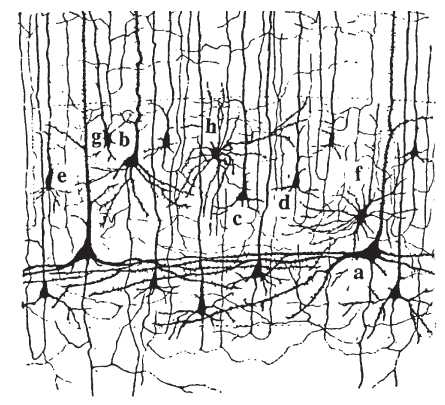
\includegraphics[width=0.4\textwidth]{imgs/brain.png} 
    \caption{A small section in the Brain. The neurons $a$ - $g$ are connected to other neurons in a complex network \cite{gerstner2014neuronal}.}
	\label{fig:brain}
\end{figure}

A human constantly brain performs tasks as learning, memory, self-control, planing, reasoning, abstract thought, motor control, vision and language.
We can localize different specialized regions in the brain which are involved in a given tasks. 

Even so different regions are involved in different tasks, the basic building blocks of the brain are astonishingly uniform. 
It is mainly composed of neurons, glial cells and blood vessels.
While the neurons cells are the main computational unit, the other constituents are required for structural stabilization and energy support.
A single neuron can perform only quite simple operations but, the human brains contains $10^{12}$ neurons and each single neuron is interconnected with $10^{4}$ other neurons.
The resulting complex neural network with roughly $10^{15}$ neural connections are the main component for human intelligence and enable complex task as scene understanding, language processing and motion planing. A small section of a neural network recorded in a human brain is shown in Figure \ref{fig:brain}. 

\subsubsection{Neuron} \label{c:natneuron}

Neurons are the main information processing unit in the brain\cite{gerstner2014neuronal}\cite{Byrne1997}. 
Information is primarily processed through chemical and electrical signals.

A neuron, which is a specialized kind of (biological) cell, is separated from its surroundings by a cell membrane.   
Due to ion concentration differences between the interior and the exterior of the cell, there are potential differences at the cell membrane, which are referred to as the membrane potential. 
Ion channels, often voltage gated, in the cell membrane allow positive and negatively charged ions to flow from the inside to the outside and from the outside to the inside of the cell.
This can lead to an increase (de-polarization) or decrease (hyper-polarization) of the membrane potential.
The ion flow is primarily determined by the charge difference at the membrane (reversal potential), the ion concentration differences (nernst potential) and ion pumps actively pumping ions across the membrane.
The membrane of a neuron at rest, with an equal influx and outflow of ions neutralizing each other, has usually a resting/equilibrium potential of -65 mV. 

Each singe neuron can be divided into three functional distinct parts: the dendrites, the soma and the synapses (see Fig. \ref{fig:neuron}).

\begin{figure}[h]
	\centering
    	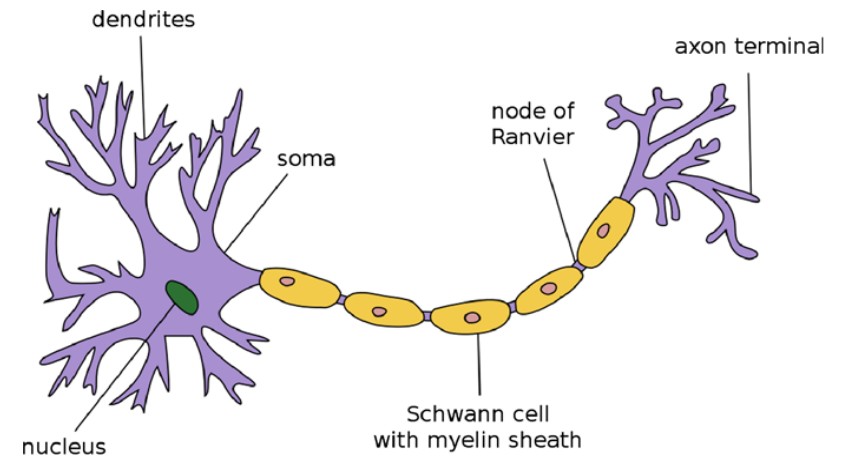
\includegraphics[width=0.6\textwidth]{imgs/neuron.png} 
    \caption{A schematic view of a natural neuron. Other neurons are pre-synaptic connected via the dendrites. The signals are then forwarded and accumulated in the soma and from there on via the in myelin sheath cover axon to the axon terminal and the out going synapses \cite{neuronImg}.}
	\label{fig:neuron}
\end{figure}

The dendrites are thin, complexly branching structures emerging the cell body/ soma.
They are the primary access for signals of preceding neurons through their synapses. 
These signals can polarize or depolarize the part of the dendrites and so inhibit or promote a spike. 

The cell body or soma, which encompasses the nucleus, accumulates all polarizations from the dendrites and if the accumulation exceeds a "pseudo" threshold, usually around -55 mV, certain ion channels become more active, which allows an influx of positively charged ions and a spike emerges.

The spike is propagated across the axon to the axon terminal where it distributed to the dendrites of other subsequent (post-synaptic) neurons via the synapses, where they in turn can evoke (post-synaptic) potentials.
The axon is often covered by a fatty substance, the myelin, to regulate and improve the conductivity.

Synapses can be divided into two different categories: Electrical, which communicate with other neurons with direct electrical connections and chemical which use chemical compounds.
Probably due to their more diverse form of signal exchange, almost exclusively all synapses found in the brain have a chemical nature.

\subsubsection{Learning} \label{c:natlearning}

The exact mechanisms behind learning in the brain are still mostly unknown \cite{gerstner2014neuronal}\cite{Byrne1997}\cite{Markram2012}.
Neural plasticity is often considered be to one of the methods behind learning. 
It describes the ability of the brain to change and reorganize the structure of brain, build new and alter connections.  

\paragraph{Synaptic Plasticity} \label{c:synplasiticity}
specifies the changes to the synaptic strength, which is often associated with task learning and memory (in contrast to learning in brain, which is the general mechanism of altering the information processing in the brain, task learning describes the actual learning and remembering of a task). 

Synaptic plasticity builds on the principle that temporally and locally correlated neural activity  can lead to synaptic changes.
It is often further divided in \textbf{short-term plasticity} which acts on a time scale one milliseconds to a minutes and \textbf{long-term plasticity}, lasting minutes or more.


\paragraph{"What fires together, wires together"} \label{c:hebb}
A principle which generalizes these principles is the Hebbian principle or Hebbian rule.
It is often commonly summarized as "Cells that fire together, wire together".
Hebb originally stated it as follows: "When an axon of cell $A$ is near enough to excite a cell $B$ and repeatedly or persistently takes part in firing it, some growth process or metabolic change takes place in one or both cells such that $A$'s efficiency, as one of the cells firing $B$, is increased."\cite{hebb19680}.
Meaning, the more often $A$ is active directly before $B$, the more likely $A$ will have contributed to $B$'s spike and the more causal $B$ will become of $A$/ $A$ and $B$ become associated.
This can be mathematically expressed as
\[
\Delta w_{ab} = \eta v_a v_b ,
\]
where $\Delta w_{ab}$ describes the change of the synaptic weight between the pre-synaptic neuron $A$ and the post-synaptic neuron $B$. 
$v_a$ and $v_b$ describe the activity of $A$ and $B$, respectively and $\eta$ is some positive learning rate. 

While this describes the classical Hebbian principle, often different algorithms processing the neural activity of two connected neurons are summarized and labelled as general Hebbian learning algorithms.
Such algorithms can in be general formalized as
\[
\Delta w_{ab} = F( v_a, v_b) , 
\]
where $F$ is a function describing the weight change conditioned on the neural activities \cite{gerstner2014neuronal}.     
This formulation allows a more complex processing of the neural activity and implementations as e.g. the original formulation of the Hebbian principle as well as the anti-Hebbian rule. 

\subsection{Artificial neural networks} \label{c:ann}

The first artificial neural network models performed computations at discrete time slices.
While it simplifies the neuron model a lot, it makes them exceptionally easy to handle on most processors, which also work at a discrete tact rate.

\subsubsection{Perceptron} \label{c:perceptron}

The perceptron, also called Rosenblatt Perceptron, was invented in the late 1950s by Frank Rosenblatt \cite{rosenblatt1958perceptron}. 
It was one of the first artificial neural networks, and can be seen as the foundation of most of the modern (deep) neural networks as well as linear discriminating classifiers. 

\paragraph{Model} \label{c:permodel}

The perceptron loosely models a neuron with a multi-dimensional input and a single output (see Fig. \ref{fig:perceptron}). 

\begin{figure}
	\centering
    	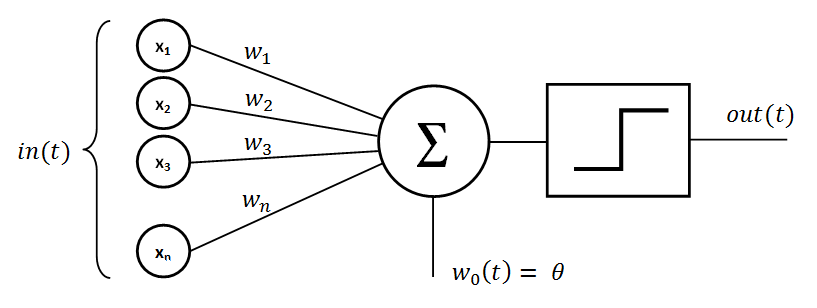
\includegraphics[width=0.8\textwidth]{imgs/percept.png} 
    \caption{Structure of a perceptron. The input $in(t)$ is set at the input variables $x_i$ and the multiplied with the corresponding synaptic weight $w_i$ and accumulated. In addition a threshold offset $\theta$ is added. On the sum the step-function is applied i.e. the output $out(t)$ is $1$ if the sum is greater $0$ and $0$ if the sum is smaller $0$ \cite{perceptronImg}.}
    % https://github.com/cdipaolo/goml/tree/master/perceptron
	\label{fig:perceptron}
\end{figure}

Be $\textbf{x} \in \mathbb{R}^n$ the input of dimension $n$ and $\textbf{w}\in \mathbb{R}^n$ the $n$-dim vector describing the synaptic weights, then each $x_i$ is multiplied by it's synaptic weight $w_i$ and then accumulated/summed up:
\[
\sum x_i w_i = \textbf{x}^\intercal \textbf{w}.
\] 

If the sum exceed a threshold $b$, often referred to as the bias, the perceptron "fires" and the output $y$ is set to $1$ and otherwise it is set to $0$.

\[
	f = 
		\begin{cases}
			1, \text{  if  } \textbf{x}^\intercal \textbf{w} + b > 0  \\
			0, \text{  if  } \textbf{x}^\intercal \textbf{w} + b \le 0
		\end{cases}	
\]

One simplification is to append the bias $b$ to the weight vector $\textbf{w}' = (b , w_1, ... , w_n)$ and to extend the input dimension by a constant one $\textbf{x}' = (1, x_1 , ... , x_n)$ .
This allows us to handle the bias as a simple synaptic weight, and thus we will cease to  model it explicitly and further on.

\[
	f = 
		\begin{cases}
			1, \text{  if  } \textbf{x}'^\intercal \textbf{w}'> 0  \\
			0, \text{  if  } \textbf{x}'^\intercal \textbf{w}' \le 0
		\end{cases}	
\]



Using the heaviside step function $\varphi_{step}$, the perceptron calculation rule can be rewritten as 
\[
	f = \varphi_{step}(\textbf{x}'^\intercal \textbf{w}) .
\]   

\paragraph{Decision Function} \label{c:perdecision}

This equation can be interpreted as a linear discrimination function, where $\textbf{w}$ defines a hyper plane in the data space, diving it into two half spaces. 
Two exemplary linear discrimination function in data space are given in Figure \ref{fig:discrimation}.
This separation of the data space into distinct sub spaces is often regarded to as classification. 
While a perceptron with a linear decision function only allows quite simple discrimination, more complex decision functions can be chosen e.g. multi layers perceptrons combine simple function into more complex ones. 

\begin{figure}
	\centering
	\begin{subfigure}[t]{.45\textwidth}
	 	\centering
  		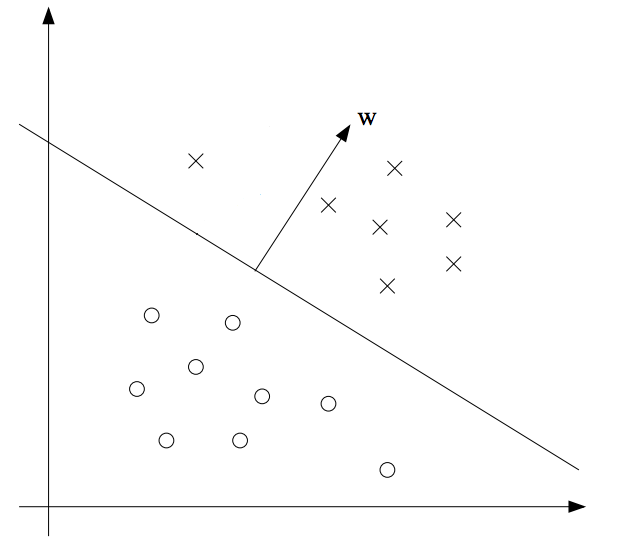
\includegraphics[width=.9\linewidth]{imgs/percept_discr1.png}
  		\caption{}
	\end{subfigure}
	\begin{subfigure}[t]{.45\textwidth}
	 	\centering
  		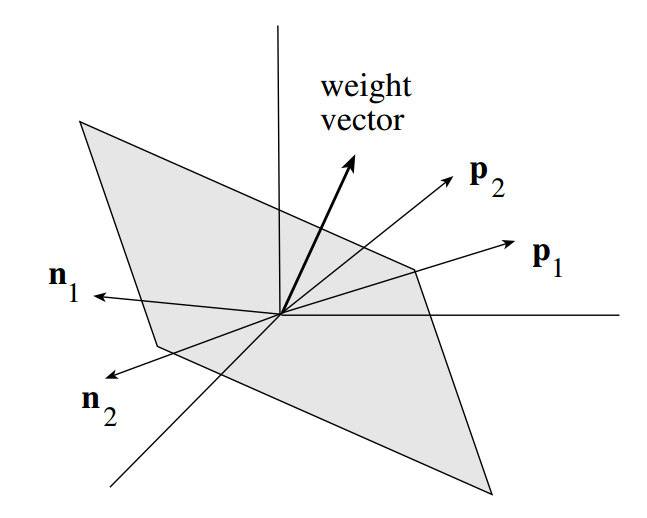
\includegraphics[width=.9\linewidth]{imgs/percept_discr2.png}
  		 \caption{}
	\end{subfigure}
    \caption{The discrimination function of a perceptron. The discrimination function has the shape of a linear hyper plane in data space and it defined by the synaptic weight-vector $\textbf{w}$. It divides the data space and thus the data samples into two subspaces, the positive space $\textbf{x}^{\intercal}\textbf{w} > 0$ and the negative space $\textbf{x}^{\intercal}\textbf{w} < 0$. In (a) the discrimination function is given in a two-dimensional data space and in (b) in a three-dimensional data space.}
	\label{fig:discrimation}
\end{figure}


\paragraph{Perceptron Learning} \label{c:perlearning}

Be $\textbf{X}$ a set of data-points and $\textbf{Y}$ their corresponding label and $\mu$ a learning rate. 

For a sample $x \in \textbf{X}$  and $y \in \textbf{Y}$ and $\tilde{y}$ the output of the perceptron, one update step can be described as:
\[ 
	w = w + \Delta w
\]
, where 
\[
	\Delta w = \mu (\tilde{y}-y) x .
\]
Thus the learning algorithm can be described as follows:

\begin{enumerate}
	\item Initialize $w$ randomly.
	\item Select a data sample and calculate its output.
	\item Calculate $\Delta w$ and update the weights.
	\item Performed steps 2.-3. until all data samples are correctly classified i.e. $\tilde{y} = y$ or a predetermined number of iterations have been completed
\end{enumerate}


\subsubsection{Mutlilayer-Perceptron} \label{c:mlp}

While the perceptron models a single neuron, a multi-layer perceptron, consisting of stacked perceptrons, can be seen as an extension of the model to neural networks and by doing so overcoming the perceptrons disadvantage to only discriminate linearly \cite{rumelhart1985learning}\cite{Goodfellow-et-al-2016-Book}. 

\paragraph{Model architecture} \label{c:mlparch}

A MLP is built up of multiple consecutive layers (see Fig. \ref{fig:mlp}).

Each layer combines multiple perceptrons to map a multi-dimensional input $\textbf{x} \in \mathbb{R}^n$ to a multi-dimensional output $\textbf{y} \in \mathbb{R}^m$.
The output $\textbf{y}$ of the layer is composed of the $m$ individual outputs $y_i$ of the perceptrons in the layer on the same input.


A layer is defined by:
\begin{enumerate}
	\item The input dimension $n$,
	\item The output dimension $m$ (which can be seen as the number of individual perceptrons in the layer),
	\item The Weight matrix $W \in \mathbb{R}^{nxm} $ defining the weights between the synaptic connections,
	\item The activation function $\varphi : \mathbb{R}^m \rightarrow \mathbb{R}^m $.
\end{enumerate}

The output $\textbf{y}$ of the layer is calculated as:
\[
\textbf{y} = \varphi(x^\intercal W)
\]

Each element $y_i \in \textbf{y}$ can be interpreted as the output of a perceptron given the input $\textbf{x}$ and the synaptic weights $w_i \in W = (w_1, ... , w_n)$.

By using the output of a previous layer $l$ as input for a next layer $l+1$, several layers can be stacked up: 
\[
\textbf{y}^{l+1} = \varphi ((\textbf{y}^{l})^\intercal W^{l+1} ) ,
\]
where the superscript index represents the layer number. 

Modelled like this, the output is always forwarded to the next layer, so there are no cycles in the information flow of the network.
Such a network with only forward connections is called feed-forward network (in contrast to recurrent networks such as Boltzmann machines, which are introduced in Chapter \ref{c:bms} and allow information to be forwarded in cycles).

\begin{figure}
	\centering
    	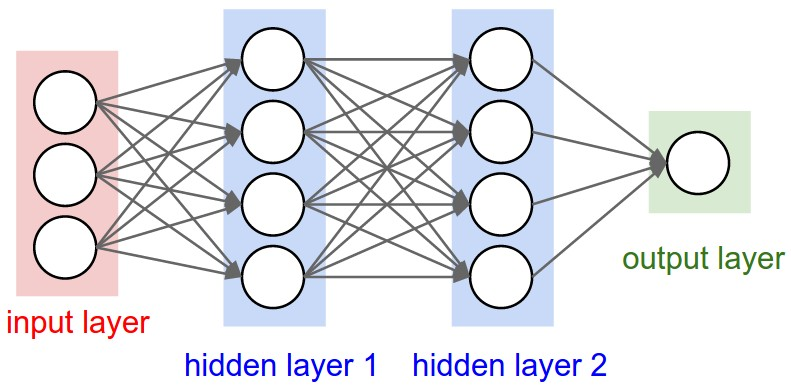
\includegraphics[width=0.6\textwidth]{imgs/mlp.jpeg} 
    \caption{A schematic multi layer perceptron with three layers \cite{mlpImg}.}
	\label{fig:mlp}
\end{figure}



\paragraph{Activation functions} \label{c:mlpact}

The activation function $\varphi$ can be basically arbitrarily chosen. 
There different activation functions, with different attributes, have been proposed, which also have proven to perform well on certain tasks:

\begin{itemize}
	\item Step-function: $\varphi_{step}(x_i) = \begin{cases} 1, & \text{if  } x_i > 0 \\ 0, & \text{if  } x_i \le 0  \end{cases}$
	\item Sigmoid-function: $\sigma(x_i) = \frac{1}{1 + e^{-x_i}}$ 
	\item Softmax-function: $\varphi_{softmax}(x_i) = \frac{e^{x_i}}{\sum_k e^{x_k}}$ 
	\item Sign-function: $\varphi_{sign}(x_i) = \begin{cases} 1, & \text{if  } x_i > 0 \\ -1, & \text{if  } x_i \le 0  \end{cases}$
	\item Tanh-function: $tanh(x_i) = \frac{e^{x_i} - e^{-x_i}}{e^{x_i} + e^{-x_i}}$
	\item ReLU-function $\varphi_{ReLU}(x_i) = max(0, x_i)$
\end{itemize}

A visualization of those functions is given in Figure \ref{fig:activations}.

\begin{figure}
	\centering
    	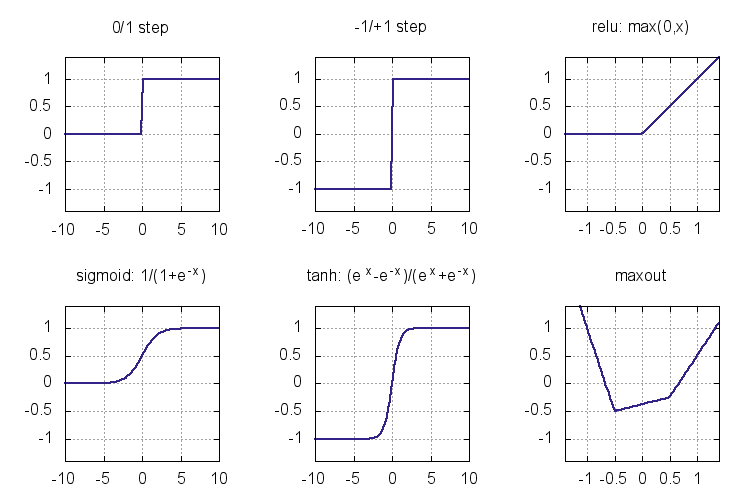
\includegraphics[width=0.8\textwidth]{imgs/act_fun.png} 
    \caption{The output of different activation functions plotted given the input.}
    % http://knet.readthedocs.io/en/latest/mlp.html
	\label{fig:activations}
\end{figure}

Different activation functions describe the behaviour of the neurons on the input data.
This is very similar to choosing different neuron models for spiking neural networks.


\paragraph{Error functions} \label{c:mlperr}

In machine learning, to validate the quality of the model an error function/cost function is used.
The error function gives a quantification of the performance of the model on a given task.
Thus the primary goal of a learning algorithm is to reduce the error on its task.
Hereby it is important to note that the main error function is often primarily task dependent and rather independent on the learning algorithm used.  

To compare the outputs $\tilde{\textbf{y}}$ of the network with parameters/weights $\theta$ to the correct data-labels $\textbf{y}$ some of the most used error function or cost function $E(\textbf{y},\tilde{\textbf{y}} | \theta)$ are:.

\begin{itemize}
	\item Mean squared error: $MSE = \frac{1}{N} \sum_{i=1}^N (\tilde{\textbf{y}}_i - \textbf{y}_i)^2 $
	\item Cross entropy: $CE = - \frac{1}{N} \sum_{i=1}^N [ \textbf{y}_i \log \tilde{\textbf{y}}_i + (1 - \textbf{y}_i) \log (1 - \tilde{\textbf{y}}_i)]$
\end{itemize}

\paragraph{Backpropagation} \label{c:backprop}

In order to reduce the error $E$ on a task, the parameters $\theta$ of the model can be changed.
This modification of the parameters is often referred to as learning.
Thus the objective is to get parameters $\theta^*$ which form a (global) minimal point in the error function. 
Different optimization algorithms can be used to achieve this objective, but the most common class of algorithms use the gradient of the error function with respect to the weights, to determine the contributions of the weights to the error and thus reduce the error and reach a minimal point.
Gradient descent calculates the gradient for the parameters, and by following the negative gradient direction the weights are updated.

Since MLPs have a clearly defined structure, using the chain rule of calculus, the gradient descent update rule can be simplified to an iterative procedure called backpropagation (backprop)  \cite{rumelhart1985learning}\cite{Goodfellow-et-al-2016-Book}.

We define the output $y_j$ of neuron $j$ as
\[
	y_j = \varphi(net_j) = \varphi(\sum_{k=1}^n w_{kj} y_k) .
\]
 
The partial derivative of the error function $E$ with respect to a weight $w_{ij}$ can be simplified by the repetitive application of the chain rule:
\[
	\frac{\partial E}{\partial w_{ij}} = \frac{\partial E}{\partial y_j} \frac{\partial y_j}{\partial net_j} \frac{\partial net_j}{\partial w_{ij}} .
\]
 
Where the single factors of the derivation can be resolved to:
\[
	\frac{\partial net_j}{\partial w_{ij}} = \frac{\partial}{\partial w_{ij}} ( \sum_{k=1}^n w_{kj} y_k ) = y_k
\]
and 
\[
	\frac{\partial y_j}{\partial net_j} =  \frac{\partial \varphi(net_j)}{\partial net_j} = \varphi'(net_j).
\]


This just leaves the first factor $\frac{\partial E}{\partial y_j}$. It can be further divided into two simple cases:
1. The neuron $j$ is in the output layer:
\[
\frac{\partial E}{\partial y_j} = \frac{\partial E(y_j)}{\partial y_j} = E'(y_j).
\] 

2. The neuron $j$ is not in the output layer and $L$ is the layer above neuron $j$:
\[
\frac{\partial E}{\partial y_j} = \sum_{l \in L}( \frac{\partial E}{\partial net_l} \frac{\partial net_l}{\partial y_j} )  = \sum_{l \in L}( \frac{\partial E}{\partial net_l} w_{jl} ).
\] 

We define 
\[
\delta_l = \frac{\partial E}{\partial net_l} = \frac{\partial E}{\partial y_l} \frac{\partial y_l}{\partial net_l} =
\begin{cases}
E'(y_l) \varphi'(net_l), & \text{  if } j \text{ is an output neuron} \\
(\sum_{k \in K} \delta_k w_{lk}) \varphi'(net_l), & \text{  if } j \text{ is not an output neuron.}
\end{cases}
\]

This all concludes to 
\[
\frac{\partial E}{\partial w_{ij}} = 
\begin{cases}
E'(y_j) \varphi'(net_j) w_{ij}, & \text{  if } j \text{ is an output neuron} \\
(\sum_{l \in L} \delta_l w_{jl}) \varphi'(net_j) w_{ij}, & \text{  if } j \text{ is not an output neuron.}
\end{cases}
\]

An update step for a weight $w_{ij}$ can now be written as
\[
w_{ij} = w_{ij} - \mu \Delta w_{ij} = w_{ij} - \mu \frac{\partial E}{\partial w_{ij}},
\]
with a learning rate $\mu$.

\subsubsection{Convolutinal Neural Networks} \label{c:cnns}

Convolutional neural networks (CNN) exploit spacial relations and the compositional structure of the input data to regularize the complexity of the neural network by putting further constrains on the architecture of those nets.
This makes them easier to train and allows greater generalization on fewer training samples.
It is implemented by having only partially connected layers with shared connection weights, instead of fully connected nets \cite{lecun1989backpropagation}\cite{Goodfellow-et-al-2016-Book}.    

\paragraph{Convolution} \label{c:convolution}

As the name suggests CNNs perform a convolution operation \cite{Goodfellow-et-al-2016-Book}. The one dimensional convolution operation $c$ is defined as
\[
c(t) = (a * b)(t) = \int_{- \infty}^{\infty} a(x)b(t-x) dx.
\]
In this equation $a$ is usually called the input and $b$ the kernel of the convolution. The result $c$ is often referred to as the feature map.

Since recorded data (e.g. images, speech) is often discretized, we extend the convolution to discrete data
\[
c(t) = \sum_{x = - \infty}^{\infty} a(x)b(t-x).
\]
Whereas convolution is originally only defined over the one-dimensional temporal dimension, it can be also applied to multiple arbitrary dimensions, e.g. two dimensional images $I$
\[
C(i,j) = \sum_m^M \sum_n^N I(m,n) K(i - m, j -n).
\]
In this case the kernel matrix $K \in \mathbb{R}^{M \times N} $ as well as the feature map $C$ also spans multiple dimensions.
A more intuitive way to rewrite this equation can be achieved by using the commutative nature of the convolution operation
\[
C(i,j) = \sum_m^M \sum_n^N I(i - m,j - n) K(m, n).
\]
Similar to the convolution is the cross correlation, which is basically a convolution without a flipped kernel
\[
C(i,j) = \sum_m^M \sum_n^N I(i + m,j + n) K(m, n).
\]
Due to this similarity the terms convolution and cross correlation are often used ambiguously (see Fig. \ref{fig:conv} for a sample cross correlation over a two dimensional input).

\begin{figure}
	\centering
    	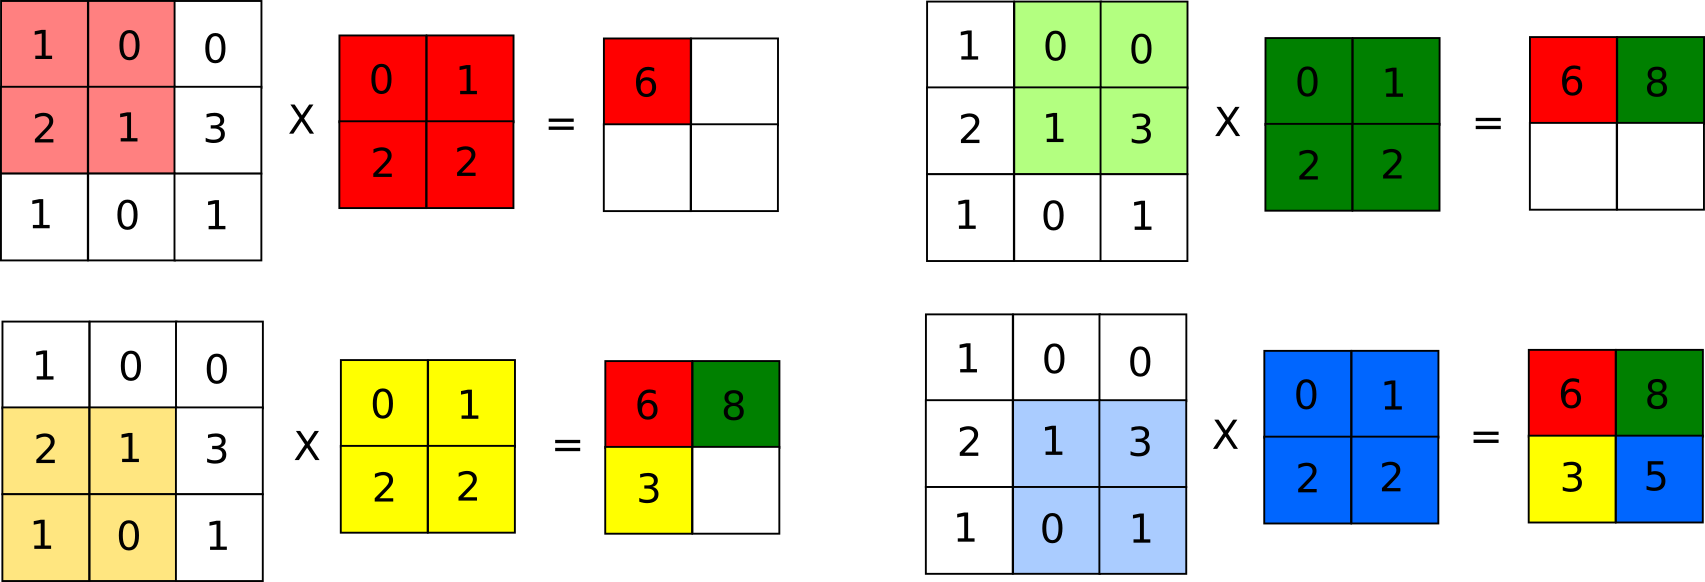
\includegraphics[width=0.8\textwidth]{imgs/convolution.png} 
    \caption{A cross correlation of a $3\times3$ image matrix with a $2\times2$ kernel without stride and padding. The result is a $2\times2$ feature map.}
	\label{fig:conv}
\end{figure}

\paragraph{Convolution Layers} \label{c:convlayers}

In neural networks convolution is implemented in the so-called convolution layer, where the convolution operation with a learnable kernel matrix $K$ is applied. An input given as an 3D tensor $Y$ be composed of $m$ 2D feature maps. Each feature map has the dimension $s \times t$. In the input layer, $m$ is for example the number of color channels (3 in case of an RGB image), and $s$ is the width and $t$ the height of the input image. A discrete convolution with a $(M , P , Q)$ filter matrix $K_j$ at position $(x,y)$ is then defined as : 
\[
y_{i}^{jxy} = \sigma(\sum_M \sum_{p=-\frac{P}{2}}^{\frac{P}{2}} \sum_{q=-\frac{Q}{2}}^{\frac{Q}{2}} w_{ij}^{mpq} y_{(i-1)}^{m(x+p)(y+q)}) .
\]
where $w_{ij}^{mpq}$ is the value at position $(m,p,q)$ of the $j$th Kernel matrix $K_j$ in the $i$th layer and $y_{i}^{jxy}$ is the entry in the $j$th 2D-feature map in the $i$th layer at position $(x, y)$.\\
In a typical layer the weights $w_{ij}^{mpq}$ of all Kernel matrices $K_j$ in all layers $i$ are the free parameters that have to be learned. Other so called hyper-parameters which have to be determined are the number $j$ of Kernel matrices at each layer $i$, their stride size, defining by how much you want to shift your filter at each step, and therefore the output dimension of the layer.
Recent state-of-the-art systems have mostly reached the common consensus, of choosing a stride of $1$, which we have adapted throughout this thesis \cite{simonyan2014very}.


%\begin{figure}
%	\centering
%	\begin{subfigure}[t]{.20\textwidth}
%  		\centering
%  		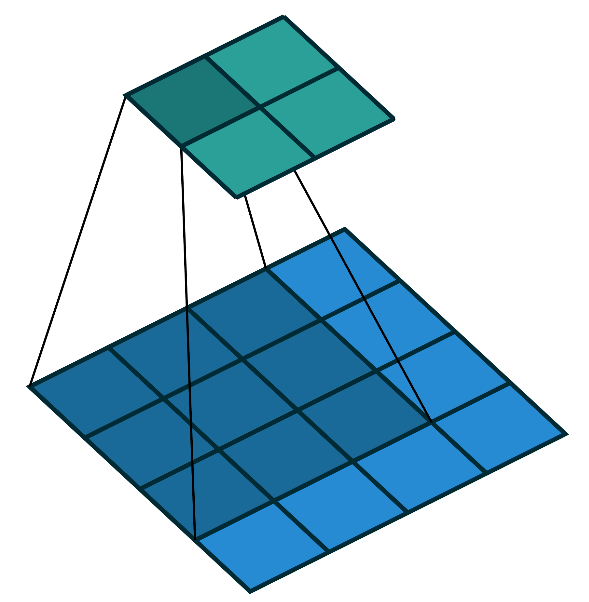
\includegraphics[width=.8\linewidth]{imgs/conv_layer1.png}
%  		\caption{A subfigure}
%  		\label{fig:sub1}
%	\end{subfigure}%
%	\begin{subfigure}[t]{.20\textwidth}
%  		\centering
%  		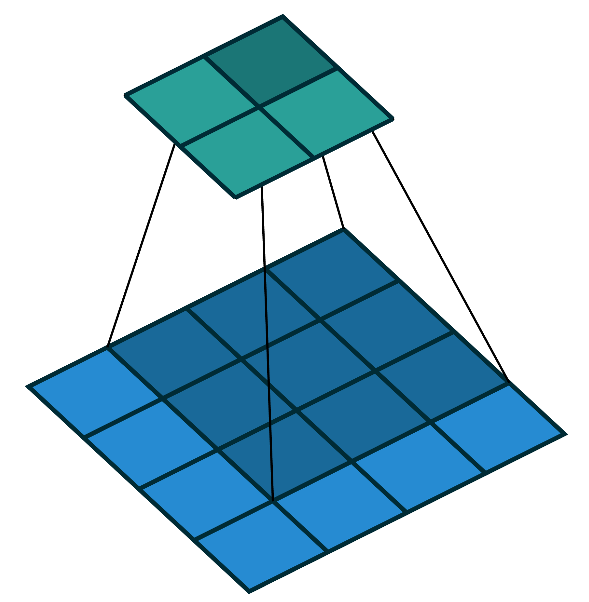
\includegraphics[width=.8\linewidth]{imgs/conv_layer2.png}
%  		\caption{A subfigure}
%  		\label{fig:sub2}
%	\end{subfigure}
%	\begin{subfigure}[t]{.20\textwidth}
%  		\centering
%  		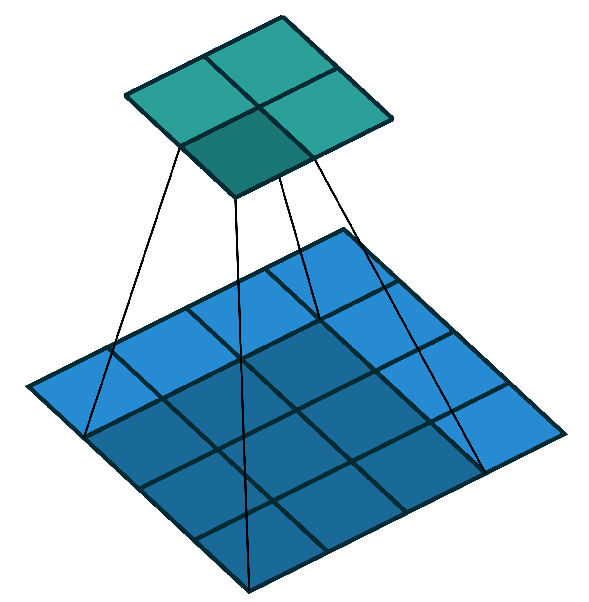
\includegraphics[width=.8\linewidth]{imgs/conv_layer3.png}
%  		\caption{A subfigure}
%  		\label{fig:sub3}
%	\end{subfigure}
%	\begin{subfigure}[t]{.20\textwidth}
%  		\centering
%  		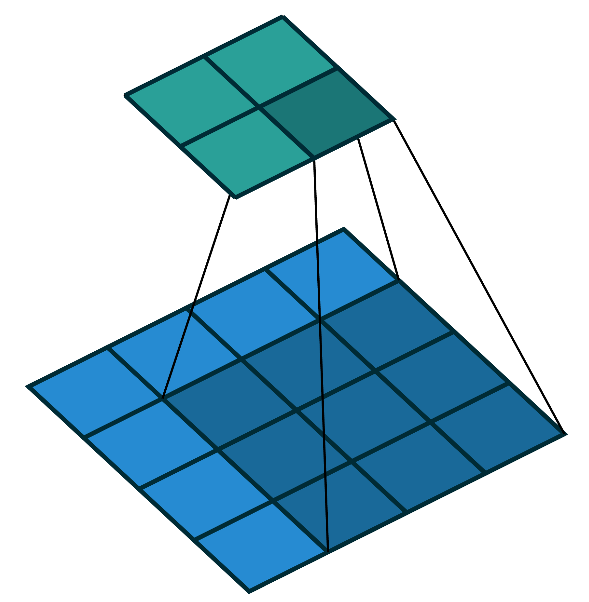
\includegraphics[width=.8\linewidth]{imgs/conv_layer4.png}
%  		\caption{A subfigure}
%  		\label{fig:sub4}
%	\end{subfigure}
%	\caption{A figure with two subfigures}
%	\label{fig:test}
%\end{figure}


\paragraph{Architecture} \label{c:cnnarch}

The most common architectures for CNNs are built up from stacks of alternating convolutional and pooling layers. 
After those layers, fully connected layers are used as a classifier to assign labels to the extracted features \cite{NIPS2012_4824}\cite{simonyan2014very}\cite{szegedy2015going}.
A sample architecture is given in Figure \ref{fig:convarcitecuture}.

\begin{figure}[h!]
	\centering
    	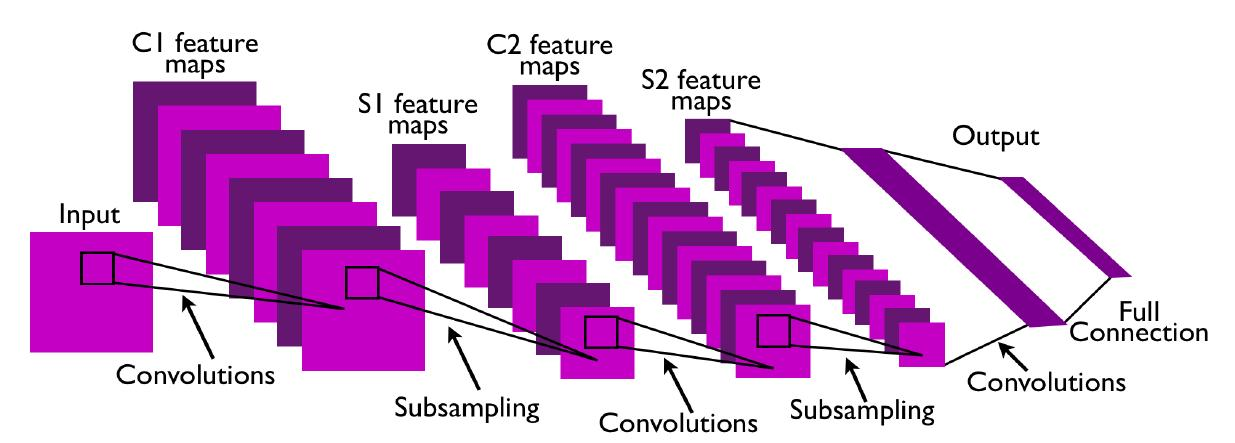
\includegraphics[width=0.8\textwidth]{imgs/cnn_architecture.jpg} 
    \caption{Typical architecture of a convolutional neural network with two convolution-pooling stages \cite{cnnarchImg}.}
	\label{fig:convarcitecuture}
\end{figure}

\paragraph{Training} \label{c:cnntraining}

% http://jefkine.com/general/2016/09/05/backpropagation-in-convolutional-neural-networks/

The training is performed applying the backprop algorithm to convolution:
\[
\frac{\partial E}{\partial w_{ij}^{mpq}} = \sum_{m'} \sum_ {q'}  \sum_{p'} \frac{\partial E}{\partial y_i^{m' p' q'}}  \frac{\partial y_i^{m' p' q'}}{\partial w_{ij}^{mpq}}  = \sum_{m'} \sum_ {q'}  \sum_{p'} \delta_i^{m' p' q'}  \frac{\partial y_i^{m' p' q'}}{\partial w_{ij}^{mpq}}.
\] 
By applying the chain rule this can be rewritten as
\[
\frac{\partial E}{\partial w_{ij}^{mpq}} = \sum_{m'} \sum_ {q'}  \sum_{p'} \delta_i^{m' p' q'}  \varphi(y_{i-1}^{m'-m, p'-p, q'-q}) = \delta_i^{m p q}  * \varphi(y_{i-1}^{-m, -p, -q}).
\] 
Another more intuitive update rule is given by defining the contribution to the error of an single weight as
\[
\frac{\partial E}{\partial y_i^{m' p' q'}}  \frac{\partial y_i^{m' p' q'}}{\partial w_{ij}^{mpq}}  = \Delta w_{ij}^{m' p' q'}.
\] 
Thus $\frac{\partial E}{\partial y_i^{m' p' q'}}$ can now be defined as
\[
\frac{\partial E}{\partial w_{ij}^{mpq}} = \sum_{m'} \sum_ {q'}  \sum_{p'} \Delta w_{ij}^{m' p' q'},
\] 
which boils down to applying the sum of each individual weights of a group of "tied" weights to all tied weights of the group.



\subsubsection{Hopfield Nets} \label{c:hopnets}

While CNNs have been wildly successful on image and speech recognition tasks, due to their pure forward nature of their connections, they still lack some biological plausibility since there are more feedback than feed-forward connections in the visual cortex .
Hopfield nets try to overcome some of those issues by using recurrent connections and binary units \cite{hopfield1982neural} \cite{Goodfellow-et-al-2016-Book} (see Fig. \ref{fig:hopfiled} for a sample net with 8 units).

\paragraph{Model} \label{c:hopmodel}

Hopfield nets use binary units, meaning each unit/neuron can be either "firing" (having value 1) or "not firing" (having value -1). 

A Hopfield net  is fully connected with recurrent connections with symmetric weights but has no self connections:
\[
\begin{split}
w_{ii} = 0 , \\
w_{ij} = w_{ji} .
\end{split}
\]

The activation of a unit is similar to perceptron with a sign activation function and depends only on its neighbour units. It is calculated using the following rule:
\[
	s_i = 
		\begin{cases}
			1, & \text{  if  } \sum w_{ij} s_{j} - b_{i}> 0 , \\
			-1, & \text{  if  } \sum w_{ij} s_{j} - b_{i} \le 0,
		\end{cases}	
\]
where $s_i$ is the current state/ activity of neuron $i$.

\begin{figure}
	\centering
    	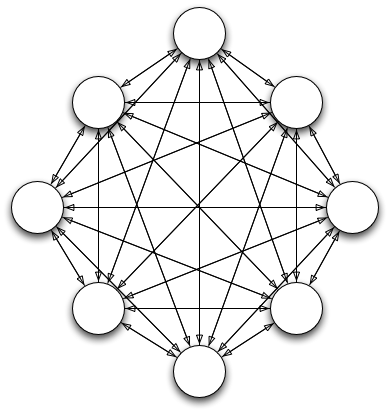
\includegraphics[width=0.5\textwidth]{imgs/hopfield.png} 
    \caption{A blueprint of a Hopfield nets with 7 binary units. The units are connected with symmetric undirected connections.}
	\label{fig:hopfiled}
\end{figure}


In contrast to feed-forward networks in Hopfield nets, there is no clearly defined bottom layer and order of the layers, thus the updates can be performed in two different way :
\begin{itemize}
\item Asynchronous: One unit is updated at a time. The units are either chosen randomly or in a predefined order
\item Synchronous: All units are updated at the same time (based on the previous states of all units)
\end{itemize}

Similar to energy based models each state $z = (s_1, ... , s_n)$ can be described by an energy, which for Hopfield nets the energy of a state is defined as  
\[
E(z) = - \frac{1}{2} \sum w_{ij} s_i s_j + \sum b_i s_i .
\]


By introducing recurrent connections, the network can be trained to store information.
Indeed, with each (asynchronous) update step the energy is thus guaranteed to stay the same or lower in value.
And thus the network will converge to a local minimum of the energy function, similar to a stable equilibrium state, where it can not escape from. 
Such a state can be called mode or attractor state.
Hopfield nets can be trained as associative memory, where each stored pattern corresponds to such an attractor state.

The training rule for associative memory is a local Hebbian rule, i.e. for an update they only use information of neurons on either side of a connection:
\[
w_{ij} = \frac{1}{n} \sum_{patterns} s_{i} s_{j}
\]

Such Hopfields net can consequently perform pattern completion by reaching a low energy state, but it can also end in a spurious state, an attractor state/local energy minimum, which was not presented as a training data.


\subsubsection{Boltzmann Machines} \label{c:bms}

Boltzmann machines try to improve Hopfield nets by replacing the deterministic update rule with a stochastic one.
This allows a more stochastic exploration of the network states due to probabilistic escaping of minima states \cite{ackley1985learning} \cite{Goodfellow-et-al-2016-Book}.

\paragraph{Model} \label{c:bmmodel}

Similar to a Hopfield net the units $s_i$ in a Boltzmann machine are binary as well and can have the value $s_i = 1$ or $s_i = 0$. 
A further similarity are bidirectional, symmetric weights without any self connections, and an equivalent energy function:
\[
	E(z) = - \frac{1}{2} \sum w_{ij} s_i s_j + \sum b_i s_i .
\]
This allows the interpretation of a Boltzmann machine as an energy based model with the probability distribution defined by the energy function $E$ and its parameters $\textbf{w}$.

A Boltzmann machine is an energy based model with the probability distribution defined by the Energy.
Thus each state $\textbf{z}$ can be assigned a Energy which is directly indicates the probability of the state $P(\textbf{z}) \propto -E(\textbf{z})$:
\[
P(\textbf{z}) = - \frac{1}{Z} \exp^{-E(\textbf{z})} 
\]

A unit is updated probabilistically given the states of its neighbour units:
\[
p_{on}(s_i) = \sigma( \sum s_j w_{ij} + b_i ), 
\]
where $\sigma$ is the sigmoid-function.

An update step can be seen as a Gibbs sampling step from the distribution defined by $E$.
Running a certain number of consecutive update steps probabilistically drives the network to a low energy or equilibrium state.


\begin{figure}
	\centering
    	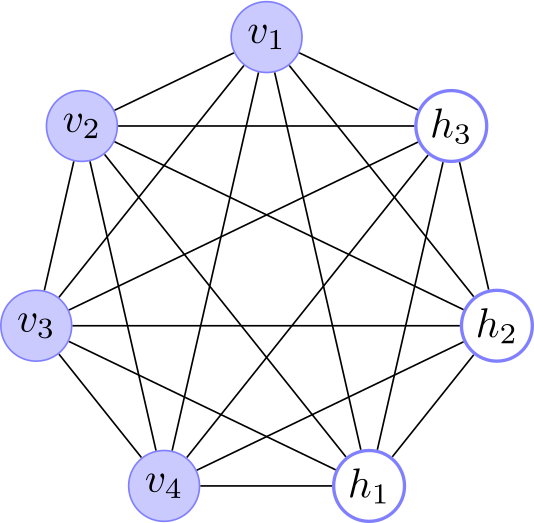
\includegraphics[width=0.5\textwidth]{imgs/bm.png} 
    \caption{A Boltzmann machine with 7 units. In contrast to a Hopfield nets, units are divided into visible and hidden/ unobserved units with stochastic activations \cite{boltzImg}.}
    % http://gorayni.blogspot.de/
	\label{fig:bm}
\end{figure}

In contrast to Hopfield nets where each unit of the network is represented by a element a data sample, in Boltzmann machines latent variables are introduced to increase the capacity of the network.
The units are thus divided into observable visible units and unobservable hidden/latent units (see Fig \ref{fig:bm}).
With hidden units a Boltzmann machine becomes a universal approximation probability mass functions over discrete variables.


\paragraph{Learning Rule} \label{c:cd}

The goal for training a Boltzmann machine is to get a probability distribution, which is similar to the distribution which generated the training data, the so-called data distribution.
Thus the objective for a Boltzmann machine is to assign a high probability to its training data (while assigning a low probability data not drawn from the data distribution) \cite{ackley1985learning} \cite{hinton2002training} \cite{Woodford2002} \cite{Bengio2009}.
By using gradient descent we will adapt the parameters/ weights of the Boltzmann machine in a directions which assigns trainings samples $\textbf{x}$ a high probability:
\[
w_{ij} = w_{ij} - \mu \Delta w_{ij},
\]
where
\[
\Delta w_{ij} = \frac{\partial P(\textbf{x})}{\partial w_ij}.
\]

By using the logarithm of the probability function $\frac{\partial P(\textbf{x})}{\partial w_{ij}}$ can be rewritten as
\[
\frac{\partial P(\textbf{x})}{\partial w_{ij}} = \frac{\partial Z}{\partial w_{ij}} - \frac{1}{K} \sum_{i=1}^K \frac{\partial \log E(\textbf{x}_i)}{\partial w_{ij}} =  \frac{\partial Z}{\partial w_{ij}} - \Big \langle \frac{\partial \log E(\textbf{x})}{\partial w_{ij}} \Big \rangle_{\text{data}}.
\]    

The derivation of the partition function $Z$ by $w_{ij}$ can be restated as
\[
 \frac{\partial Z}{\partial w_{ij}} = \int p(\textbf{x}) \frac{\partial \log E(\textbf{x})}{\partial w_{ij}} dx = \Big \langle \frac{\partial \log E(\textbf{x})}{\partial w_{ij}} \Big \rangle_{\text{model}}.
\]

Thus the update rule is now given as
\[
\frac{\partial P(\textbf{x})}{\partial w_ij} =  \Big \langle \frac{\partial \log E(\textbf{x})}{\partial w_{ij}} \Big \rangle_{\text{model}} - \Big \langle \frac{\partial \log E(\textbf{x})}{\partial w_{ij}} \Big \rangle_{\text{data}}
\]
The derivation of $\log E$ after a weight $w_{ij}$
\[
\frac{\partial \log E(\textbf{x})}{\partial w_{ij}} = s_i s_j
\]

gives the quite simple update rule called contrastive divergence (CD)
\[
w_{ij}= w_{ij} + \mu ( \langle s_i s_j \rangle_{\text{data}} - \langle s_i s_j \rangle_{\text{model}} ) ,
\]
where $\langle s_i s_j \rangle_{\text{data}}$ are the expected activations from the data distribution and  $ \langle s_i s_j \rangle_{\text{model}}$ are the expected activations from the model distribution.
The most common way to get the data and model distribution is to perform consecutive Gibbs update steps until an equilibrium distribution is reached, with either training data clamped or no data clamped to visible units.

Here $\langle s_i s_j \rangle_{\text{data}}$ is referred to as the positive phase and $ \langle s_i s_j \rangle_{\text{model}}$ as negative phase.
A simple interpretation of the update rule is a shift of the weights away from the model distribution towards the data distribution.

\subsubsection{RBMs} \label{c:rbms}

To perform such an update, samples from the model distribution are needed. 
To get those samples, the Boltzmann machine has to reach an equilibrium distribution. 
This can be quite computationally expensive and there is no guarantee to tell when the equilibrium distribution is reached.
Thus potentially infinite sampling steps have to be performed.

To evade the problem, a simple solution is to make the hidden units not dependent on each other (and the visible not dependent on each other), so all hidden units can be sampled independent and parallel of each other.
Thus a Boltzmann machine with two bipartite layers is called restricted Boltzmann machine (RBM) (see Fig. \ref{fig:rbm}) \cite{smolensky1986information}.

Sampling the hidden units $\textbf{h}$ given the visible units $\textbf{v}$ is called a \textit{upward pass} and sampling the visible units $\textbf{v}$ given the hidden units $\textbf{h}$ is called a \textit{downward pass}.

In this case the probability of data sample $\textbf{x}$ can be expressed using the free energy $F(\textbf{v})$ over its visible activations $\textbf{v}$ \cite{hinton2010practical}\cite{Fischer2014}:
\[
p(\textbf{x}) =  p(\textbf{v}) = \sum_{\textbf{h}} \exp^{-E(\textbf{v},\textbf{h})} = \exp^{-F(\textbf{v})},
\]
where the free energy can also be expressed as
\[
F(\textbf{v}) = - \sum x_i b_i - \sum \log(1 + \exp^{x_i})  .
\]

\begin{figure}
	\centering
    	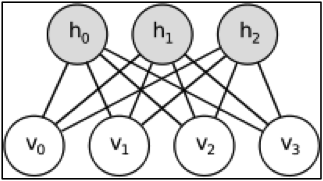
\includegraphics[width=0.5\textwidth]{imgs/rbm.png} 
    \caption{A restricted Boltzmann machine is special kind of Boltzmann machine with no lateral connections in the hidden and visible layer. This eases sampling, since the visible are only dependent on the hidden units and the hidden units only on the visible units \cite{theanoRBM}.}
	\label{fig:rbm}
\end{figure}

\paragraph{CD-k Training} \label{c:cdk}

The simplified structure of an RBM enables faster weight updates. 
Hinton showed empirically that this training procedure can be further improved by running only a limited number of Gibbs sampling steps to approximate the model distribution \cite{hinton2002training}.

The gradient calculated with this approximation can be seen as "good enough" to perform updates, which drive the underlying distribution towards the data distribution.

Thus given a data sample $\textbf{x}$ an CD-k update is computed as follows:
\begin{enumerate}
\item Perform one upward pass given $\textbf{v}_0=\textbf{x}$ to get $\textbf{h}_0$.
\item Perform k alternating downward and upward passes to get $\textbf{v}_k$ and $\textbf{h}_k$.
\item Update $w_{ij} = w_{ij} + ( (s_i s_j)_0 - (s_i s_j)_k ) $ 
\end{enumerate} 

\begin{figure}
	\centering
    	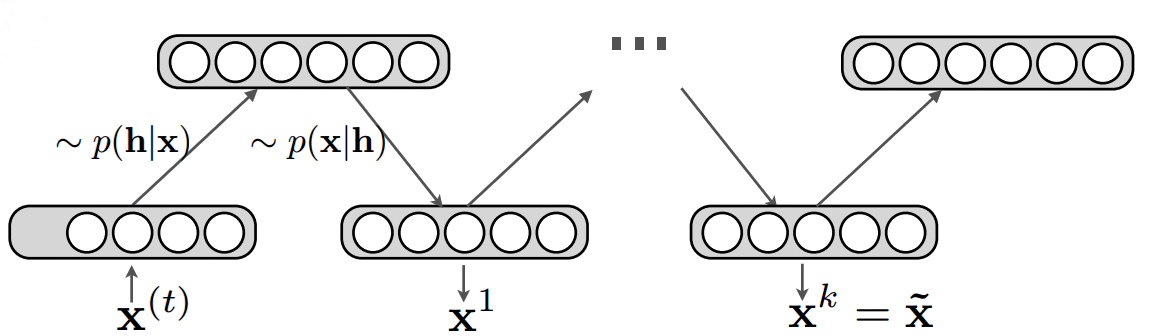
\includegraphics[width=0.8\textwidth]{imgs/cd.png} 
    \caption{A temporal unrolling of the contrastive divergence algorithm with $k$ sampling step. The hidden units and the visible units are alternatingly sampled conditioned on the current state of the other \cite{cdImg}.}
	\label{fig:cd}
\end{figure}

In Figure \ref{fig:cd} the sampling steps are visualized by unrolling the RBM as a directed model.

\paragraph{Persistent CD} \label{c:pcd}

, proposed by Tieleman, does not initialize the Boltzmann machine new each time a new sample is drawn, but uses the activations of previous runs instead \cite{tieleman2008training}. An intuition why it sometimes shows better performance could be that the previous activations are already closer to an energetic minimum, so that fewer step are required to get an good estimate of the model distribution. 


\subsubsection{Deep Belief Networks} \label{c:dbns}

A deep belief network (DBN) is a generative graphical model, or alternatively a type of deep neural network, composed of multiple layers of latent variables (hidden units), with connections between consecutive layers, but with no connections within layer \cite{hinton2006fast} \cite{hinton2009deep} \cite{Goodfellow-et-al-2016-Book}.

A deep belief network can be built up by stacking up RBMs.
This does not only enable unsupervised training of a deep belief net, but also improves the conditional distribution of the bottom RBM (each time a RBM is added, it improves the prior over the hidden units with a better and more complex prior).

In a deep belief net the two top layers form a RBM with symmetric weights while the weight symmetry can be broken up between the lower layers to allow unsymmetrical weights.   

\paragraph{Training} \label{c:dbntraining}

Training of a DBN can be split up into greedily training simple RBMs on a cascade of stacked up RBMs (see Fig. \ref{fig:dbn}).
The training procedure can be formalized as:  
\begin{enumerate}
\item Train a new top RBM given the transformed data from the bottom layers
\item After training one RBM, transform the training data by sampling the hidden layer activations of the top RBM
\end{enumerate}

After training, the DBN still has symmetric weights. 

\begin{figure}
	\centering
    	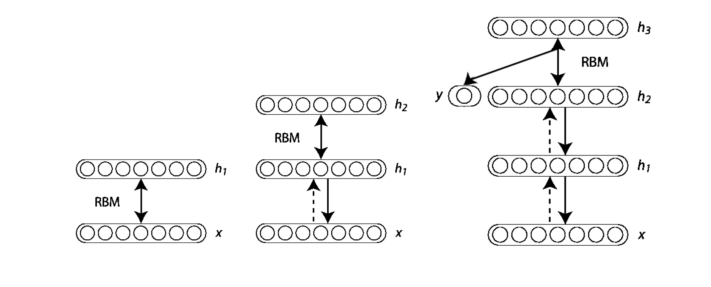
\includegraphics[width=0.8\textwidth]{imgs/dbn_stacking.png} 
    \caption{Building up a deep belief network, by training RBMs greedily and stacking them up on top of each other. At first only one RBM is trained. On top of the first RBM the next RBM is trained. This can procedure can be performed for an arbitrary number of repetitions. In the top layer "association" RBM the label information $y$ can be in-cooperated as well \cite{DBNImg}.}
	\label{fig:dbn}
\end{figure}

\paragraph{Fine-tuning} \label{c:dbnfinetuning}

After greedily training the DBN, the bidirectional connections can be split up and fine tuned to a certain task.
In general there are two most used fine-tuning algorithms, the wake-sleep algorithm for data generation and the backprop algorithm for classification. 

In the wake-sleep algorithm the symmetric weights are split up into bottom-up and top-down weights and are fine-tuned individually \cite{hinton1995wake}
\begin{enumerate}
\item Do a stochastic forward pass, and for each layer adjust the top-down weights, to better reconstruct the activations in the layer below.
\item Perform sampling steps in the top level RBM and adjust the weights with CD.
\item Do a stochastic backward pass, and for each layer adjust the bottom-up weights, to better reconstruct the activations in the layer above.
\end{enumerate}

Another way to fine-tune the weights for classification given labels and an error function, is to perform back propagation to further fine tune the bottom-up weights (while the top-down weights are usually discarded). 
One interpretation of this is to see a DBN as a pre-trained ANN.

\subsection{Spiking neural networks} \label{c:snns}

While all the previous presented models did run at discrete time steps, the next models are designed to run contentiously which makes them more similar to natural neurons and neural networks \cite{maass1997networks}. 

\subsubsection{Neuron Models} \label{c:snnneurons}

Similar to the activation function in ANNs, in SNNs there are also different models describing how neurons process input.
Most neuron models describe the development of a neuron's membrane potential over time.
Therefore the models commonly have a resting potential, which describes the membrane potential a rest without any external influences. 
Most models also have a way to model external input from incoming spikes and an internal leakage pulling the membrane potential back to its resting potential. 
If a "pseudo" threshold is exceeded usually a spike is emitted and the neuron reaches a refractory phase for some time.

\paragraph{LIF} \label{c:lif}

The leaky integrate and fire (LIF) neuron is a neuron model, which phenomenological describes the membrane potential at the soma \cite{abbott1999lapicque}\cite{gerstner2014neuronal}\cite{Petrovici2016}. 
It is one of the simplest and thus computationally most efficient, most important and popular spiking neuron models.  

\begin{figure}
	\centering
    	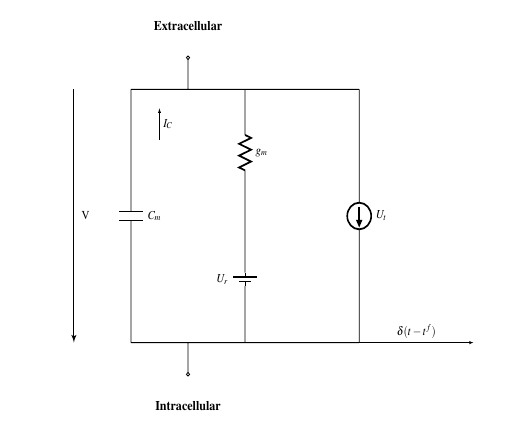
\includegraphics[width=0.6\textwidth]{imgs/lif.png} 
    \caption{A LIF neuron as an electrical circuit. The capacitor $C_m$ corresponds to the potential at the membrane, $g_l$ the leakage potential and $E_l$ the resting potential. If the membrane potential is greater than $U_t$ a spike $\delta$ is emitted \cite{heikoMA}.}
    % Heiko
	\label{fig:lif}
\end{figure}

By discarding the different forms/shapes of the action potentials and reducing it the uniform spike events, the information in condensed to the precise spike times.
The model, described by linear equations, models the membrane potential integration due to spike input currents with a capacitor and introduces a leaky current with a resistor. 
The model can be represented by a circuit of a single capacitor and a resistor with a battery (see Fig. \ref{fig:lif}):
\[
C_m \frac{\partial u}{\partial t} = g_l ( E_l - u(t) ) + I^{syn} + I^{ext} , 
\]
where $C_m$ is the membrane capacitance, $g_l$ is the leak conductance, $E_l$ the resting potential and the input current $I = I^{syn} + I^{ext}$ is divided into a static external input $I^{ext}$ and a synaptic input $I^{syn}$.   

If the membrane potentiality exceeds a threshold $\theta$ a spike $s$ is emitted and the membrane potential is instantaneously pulled back to it's reset potential $u_{reset}$ and kept at this potential for its refractory period $t_{ref}$.
\[
u(t_{s} < t \le t_{s} + t_{ref}) = u_{reset}.
\]

The emitted spikes are modelled as a spike train $\rho$ using only the precise spike times:
\[
\rho(t) = \sum_{\text{spikes } s} \delta(t-t_s),
\] 
where $\delta$ is the Dirac delta function.

Due to its simplifications the LIF model can not capture some natural observed behaviour such as bursting or adaptation (see Fig. \ref{fig:neuronbe}). 

\begin{figure}
	\centering
	\begin{subfigure}[t]{.32\textwidth}
	 	\centering
  		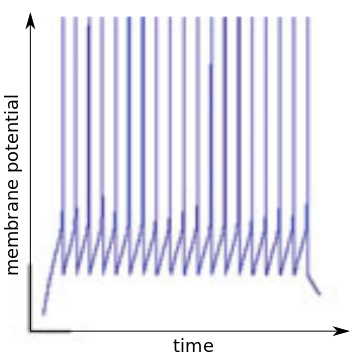
\includegraphics[width=.9\linewidth]{imgs/lif_bad1.png}
  		\caption{Constant tonic firing}
	\end{subfigure}
	\begin{subfigure}[t]{.32\textwidth}
	 	\centering
  		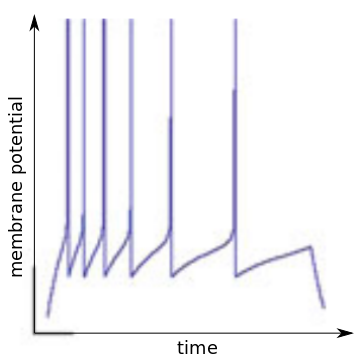
\includegraphics[width=.9\linewidth]{imgs/lif_bad2.png}
  		\caption{Frequency adaptation}
	\end{subfigure}
	\begin{subfigure}[t]{.32\textwidth}
	 	\centering
  		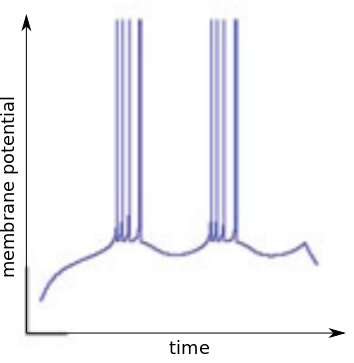
\includegraphics[width=.9\linewidth]{imgs/lif_bad3.png}
  		\caption{Delayed regular bursting}
	\end{subfigure}
    \caption{Different firing behaviour observed in the Brain. In (a) a neuron shows constant tonic firing, while in (b) the neuron shows frequency adaptation and in (c) the neurons shows delayed regular bursting \cite{gerstner2014neuronal}.}
	\label{fig:neuronbe}
\end{figure}



\paragraph{Hodgkin-Huxley} \label{c:hodghux}

The Hodgkin-Huxley model tries to improve some of the limitations of the LIF model, by explicitly allowing to model different ion channels \cite{Hodgkin1952}\cite{gerstner2014neuronal}. 

The first model described by Hodgkin-Huxley introduced three different ion channels, namely sodium, potassium and a leak current of $\text{CL}^{-}$ ions, which they discovered in their experiments on axon of a squid.
Each channel is described as a resistor with a battery (see Fig. \ref{fig:hogdehux}).
The Hodgkin-Huxley model with three ion channels can be described by the following equations :
\[
C_m \frac{\partial u}{\partial t} = g_{Na} m^3 h (E_{Na} - u(t)) + g_K n^4 (E_K - u(t)) + g_l (E_l - u(t)) + I,
\]

where the variables $h$, $m$, $n$  are described by :
\[
\begin{split}
	\frac{\partial h}{\partial t} = \alpha_h u(t) (1-h) - \beta_h u(t) * h , \\
	\frac{\partial m}{\partial t} = \alpha_m u(t) (1-m) - \beta_m u(t) * m , \\
	\frac{\partial n}{\partial t} = \alpha_n u(t) (1-n) - \beta_n u(t) * n ,
\end{split}
\]
with the rate constants $\alpha$, $\beta$ for each ion channel.

\begin{figure}
	\centering
    	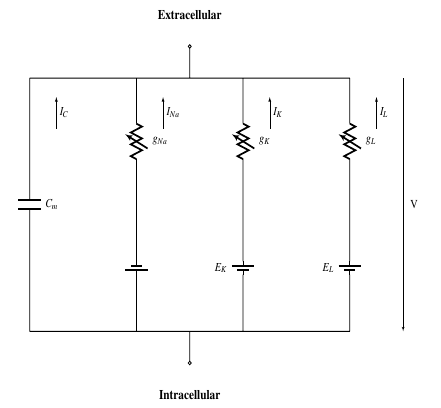
\includegraphics[width=0.6\textwidth]{imgs/hode_hux.png} 
    \caption{A Hodgkin-Huxley as an electrical circuit. The membrane potential corresponds to $C_m$, and the ion channels to $g_{Na}$, $g_{k}$, $g_{L}$ with their reversal potentials $E_{Na}$, $E_{}$, $E_{L}$ \cite{heikoMA}.}
    % Heiko
	\label{fig:hogdehux}
\end{figure}

This model can be extended/generalized to model more than three ion channels with their dynamics, to better match the characteristics/biophysics of different neurons in the brain:
\[
C_m \frac{\partial u}{\partial t} = \sum_{k \in K} g_k m^{p_k} h^{q_k} (E_k - u(t)) + I,
\]
with an arbitrary number of ion channels $K$.

While this allows the model to predict and simulate various effects observed in the brain, like frequency adaptation, with high accuracy, the Hodgkin-Huxley model is more computationally expensive.

\paragraph{Activity in a network} \label{c:poissonspikes}

One way to introduce activity into a spiking neural network is to use a Poisson spike generator \cite{Heeger2000}.
A Poisson spike generator produces stochastic firing according to a Poisson point process.
The firing rate $\lambda$ or rate function $\lambda(t)$ determines the dynamics of the homogeneous or inhomogeneous Poisson process respectively and thus of the spike times.   

The probability of a emitted spike in an time interval $\delta t$ is given by: 
\[
P_{spike}({t , t+ \delta t}) = \lambda(t) \delta t,
\]
where the occurrence of a spike is independent on previous spikes. 

Since the spikes can be formalized as a Poisson process, the expected number of spikes for an time interval $\delta t$ is given by :
\[
\langle  P_{spike}({t , t+ \delta t}) \rangle = \int_t^{t + \delta t} \lambda(t) dt.
\]


\subsubsection{Synapses} \label{c:synapses}

While synapses in ANNs are simply multiplying an incoming input with their weights, for SNNs there are different models which add additional dynamics to closer model naturally observed behaviour. 

The behaviour of the synapses are described by modelling the synaptic input $f^{syn}$. A basic model of how the influence of synapses can be described as follows \cite{Petrovici2016}:
\[
f^{syn}(t) = \sum_{\text{synapses } k } \sum_{\text{spikes } s} w_k \varepsilon(t - t_s),
\]
where $\varepsilon$ is a function describing the spike shape of the post synaptic potential (PSP).
Different shapes will discussed in the paragraph \textit{Kernel functions} \ref{c:pspkernel}.

\paragraph{Current-based synaptic interaction} \label{c:cuba}
One synapse type models the input current of neuron $I^{syn}$ directly as the synaptic input $f^{syn}$. This is a logical implementation for LIF neurons since they directly model the potential at the soma and don't consider most of the membrane dynamics in the dendrites. 
Thus the synaptic input current is given as a linear summation of the post synaptic potentials with temporal effects:
\[
I^{syn}(t) = \sum_{\text{synapses } k } \sum_{\text{spikes } s} w_k \epsilon(t - t_s),
\]
where $\epsilon$ is a kernel describing the explicit shape of a post synaptic spike.

\paragraph{Conductance-based synaptic interaction} \label{c:coba}
Conductance-based synapse models describe the synaptic dynamics more closely to its natural counterpart. They consider the conductance changes of incoming spikes, which push the conductance locally towards the reversal potential of the specific ion type. 

In this case the synaptic input $f^{syn} $can be seen as a change in the synaptic membrane conductance $g^{syn}$ :
\[
g_x^{syn} = \sum_{\text{synapses } k } \sum_{\text{spikes } s} w_k \epsilon(t - t_s) \text{ ,      } x \in \{e, i\}.
\]

Thus the synaptic input current $I^{syn}$ can now be described using the membrane conductance by applying Ohm's law:
\[
I^{syn}(t) = g_e^{syn} (E_e^{rev} - u(t)) + g_i^{syn} (E_i^{rev} - u(t)),
\]
where $E_e^{rev}$ and $E_i^{rev}$ is the excitatory and inhibitory reversal potential of the membrane, which can be e.g. chosen as $E_{Na}$ and $E_{K}$ respectively.  

\subparagraph{High conductance state} \label{c:hcs}
One interesting property of conductance based neurons is, that they can reach a so-called high conductance state (HCS) \cite{Petrovici2016}. Such a state is defined by a high total membrane conductance 
\[
g^{tot} = g_l + \sum_{\text{synapses } k} g_k^{syn},
\]
with 
\[
\sum_{\text{synapses } k} g_k^{syn} =: g^{syn} >> g_l .
\]
Such a state can be reached by a lot of incoming synaptic firing. e.g. high frequency Poisson noise from other neurons. 

The HCS is especially interesting, because the dynamics of the membrane potential can be described by a Gaussian process called Ornstein–Uhlenbeck process, with a mean primarily determined by the effective synaptic input (with the noise) and the variance by the total membrane conductance (see Fig. \ref{fig:ornuhl}).
In addition Petrovici showed, that in such a state the time the neuron needs to get from its resting potential to a value given by Ornstein–Uhlenbeck process can basically be neglected (see Fig. \ref{fig:hcs}).
This will show further application as a stochastically firing neuron model used for neural sampling  in Chapter \ref{c:snnsampling}.

\begin{figure}
	\centering
    	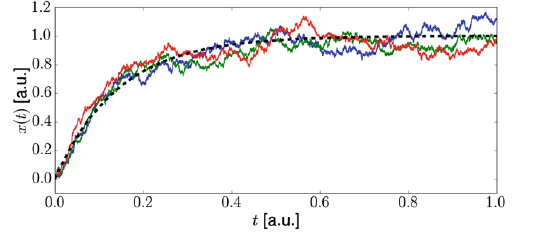
\includegraphics[width=0.6\textwidth]{imgs/orn_uhl_process.png} 
    \caption{Three samples of Ornstein–Uhlenbeck processes. This can be seen as the membrane potential of neurons in a high conductance state (in comparison to the black doted line can be seen as a neuron without noisy input) \cite{Petrovici2016}.}
    % Petrovici
	\label{fig:ornuhl}
\end{figure}


\begin{figure}
	\centering
    	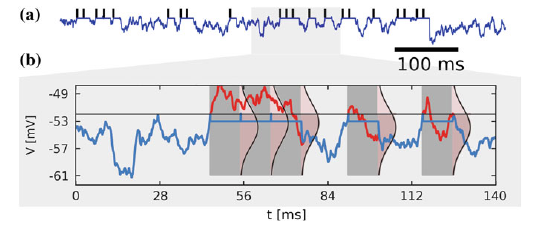
\includegraphics[width=0.6\textwidth]{imgs/hcs.png} 
    \caption{A membrane potential trajectory of a neuron in a high conductance state. (a) The spike train and the membrane potential. (b) The blue curve represents the actual membrane potential with refractory periods after each spike, while the red curve represents a membrane potential without a firing threshold. It is apparent, that the blue curve returns the the hypothetical red potential without a "return from rest" time  \cite{Petrovici2016}. }
    % Petrovici
	\label{fig:hcs}
\end{figure}


\paragraph{Kernel function} \label{c:pspkernel}

Next to the synaptic models, the kernel function $\epsilon$ has probably the most important part in modelling the synaptic input current $I^{syn}$. 
The kernel describes the explicit shape of the post synaptic potential over time and thus the influence it has on the membrane potential.
There have been several different kernel proposed, whereof some of the most important are:
\begin{itemize}
\item Rectangular-shaped: \[\epsilon(t) \propto  \begin{cases} 1, & \text{ if } t_{s} < t \le t_{s} + t_{ref} \\ 0, & \text{ otherwise } \end{cases} \]
\item Exponential-shaped: $\epsilon(t) \propto t \exp(- \frac{t}{\tau_syn})$
\item Alpha-shaped: $\epsilon(t) \propto \exp(- \frac{t}{\tau_syn})$
\end{itemize}

These are also visualized in Figure \ref{fig:pspkernels}.

\begin{figure}
	\centering
    	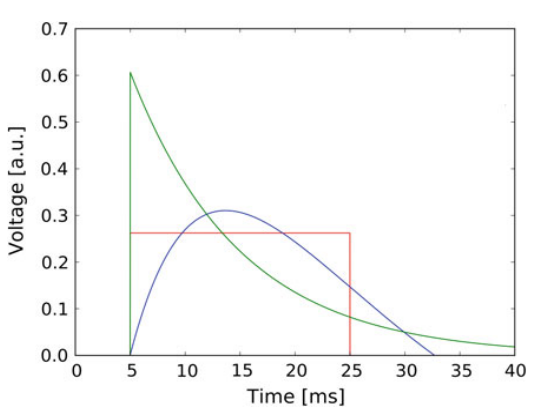
\includegraphics[width=0.6\textwidth]{imgs/psp_kernel.png} 
    \caption{Three different PSP kernels. The green one has an alpha-shape, the blue one is exponential shaped and the red one is rectangular \cite{Petrovici2016}. }
    % Petrovici
	\label{fig:pspkernels}
\end{figure}

\subsubsection{Neural Coding} \label{c:neuralcoding}

Spikes are the primary way of information transmission in the brain.
In neural networks this information can be encoded in different ways.
We will present three encoding mechanisms, which were observed in the brain, rate coding, temporal coding and population coding \cite{Meftah2013}.

In the \textit{rate coding} scheme the information is purely contained in the spike frequency/ firing rate of a neuron.
In contrast to rate coding, in \textit{temporal coding} the information is additionally transmitted via the different points in time at which the spikes are transmitted. 
Thus the information is carried in the exact spike timings.
\textit{Population coding} encodes information as the joint activity of several neurons in a population.  

In this thesis we use temporal or rate encoded input data, which is in the network represented as a population coded state over the joint activity of several neuron and is decoded in a rate-based manner. 

\subsubsection{Learning} \label{c:snnlearning}

Learning in the brain describes the generalized term, how information in the brain is stored (in contrast to task learning, memory adaptation is also considered learning).

Most models of learning algorithms in spiking neural networks build on changes in the synaptic weights/ strength between neurons to store information \cite{gerstner2014neuronal}.
To consider these changes as learning, they have to span over minutes to days or more, which is described by long term plasticity, e.g by LTP (long-term potentiation), LTD (long-term depression) or STDP (see Fig. \ref{fig:stdp}).
 
The models most commonly used are inspired on the research and discoveries of Hebb and the previously discussed Hebb principle (Chapter \ref{c:hebb}).

\paragraph{Spike time dependent plasticity} \label{c:stdp}

Spike time dependent plasticity (STDP), inspired by research on single neurons with artificially induced current, describes such a Hebbian learning algorithm.

Experiments indicated an increase of the synaptic weight if a post-synaptic spike occurred in strong temporal vicinity after a pre-synaptic spike and a decrease of the synaptic weight if a post-synaptic spike occurred in strong temporal vicinity before a pre-synaptic spike.
The further apart the spike times of the different neurons were, the weaker was the effect on the spike (see Fig. \ref{fig:stdp}).

Given the spike times of the pre- and post-synaptic neurons $t^{pre}$ and $t^{post}$, this leads to the following update rules \cite{gerstner2014neuronal}\cite{Sjostrom2010}
\[
\Delta w_{ij} = \sum_{f=1}^N \sum_{n=1}^N W(t^{post}_n - t^{pre}_f),
\]
with a common choice for the STDP function $W$
\[
W(x) =
\begin{cases}
A_+ \exp(\frac{-x}{\tau_+}) \quad \quad &\text{for  } x > 0,  \\
-A_- \exp(\frac{x}{\tau_-}) \quad \quad &\text{for  } x < 0,
\end{cases}
\]
given time constants $\tau_+$ and $\tau_-$ and the weight depend parameters $A_+$ and $A_-$.
     

\paragraph{Long-term potentiation} \label{c:ltp}
 
Long-term potentiation (LTP) can be interpreted as a STDP variant with only the positive part of the STDP function
\[
W(x) =  A_+ \exp(\frac{-x}{\tau_+}).
\]

This leads to a purely positive increase of weights (see Fig. \ref{fig:stdp}).

\paragraph{Long-term depression} \label{c:ldp}

Long-term depression (LTD) can be seen a the negative counterpart to LTP, with an STDP function
\[
W(x) =  -A_- \exp(\frac{x}{\tau_-}).
\]

This leads to a purely negative decrease of weights (see Fig. \ref{fig:stdp}).

\begin{figure}
	\centering
    	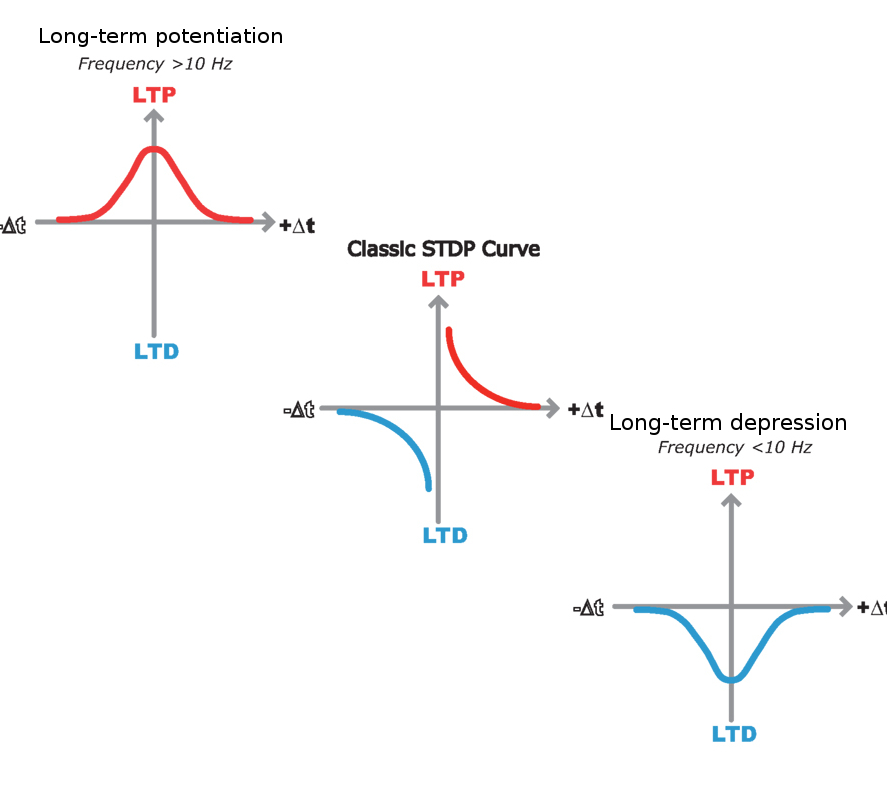
\includegraphics[width=0.6\textwidth]{imgs/stdp_curves.jpg} 
    \caption{Different STDP curves observed in the Brain. The first curve shows only long term potentiation. The middle one shows a variant of the classic STDP Curve and the last one shows purely long term depression \cite{Buchanan2010}.}
	\label{fig:stdp}
\end{figure}